\section{Introduction}
\label{s:introduction}
\todo{add decay vs erosion definition}
%%%%%%%%%%%%%%% Background Starter %%%%%%%%%%%%%%%%%%%%%%%%%%%%%%
% Due to insufficient architectural awareness, evolution can introduce architectural violations, such as architectural drift and decay, which degrade architectural integrity over time \cite{decay_icsa18,woods_ContinuousArchitecture_2021,ford_SoftwareArchitecture_2021}.  
% In practice, these violations often manifest as \acp{AS} and anti-patterns (e.g., cyclic dependencies, god components, feature concentration, microservice bad smells) \cite{fontana_2017,taibi_DefinitionMicroservice_2018}. 
% The accumulation of \ac{AS} contributes to architectural decay and to the buildup of architectural technical debt \cite{li_SystematicMapping_2015}. 
% Studies report that architectural decay is widespread and has a measurable impact on maintainability and costs \cite{sas_ArchitecturalTechnical_2023, ampatzoglou_FinancialAspect_2015,martini_ArchitectureTechnical_2014,taibi_DefinitionMicroservice_2018}.
% Existing empirical studies have shown that smells evolve over time, tending to grow larger \cite{sas_investigating_2019,sas_2022_evolution}.
% Therefore, defending against architectural decay is an important task.
Software architecture shapes how systems evolve \cite{bass_SoftwareArchitecture_2021,woods_ContinuousArchitecture_2021,bogner_assuring_2019,garlan_evolution_2009,muccini_software_2021,breivold_systematic_2012}.
Due to insufficient architectural awareness, evolution can introduce architectural violations, such as architectural drift and decay, which degrade architectural integrity over time \cite{decay_icsa18,woods_ContinuousArchitecture_2021,ford_SoftwareArchitecture_2021}.  
In practice, decay often manifests as \aclp{AS} and anti-patterns. 
Instances of architectural smells are sets of components together with a smell type, (e.g., cyclic dependencies, god components, feature concentration, microservice bad smells) \cite{fontana_2017,taibi_DefinitionMicroservice_2018,ntentos_2023}.
Architectural smells accumulate as architectural technical debt \cite{li_SystematicMapping_2015}, measurably impacting maintainability and costs \cite{sas_ArchitecturalTechnical_2023,ampatzoglou_FinancialAspect_2015,martini_ArchitectureTechnical_2014,taibi_DefinitionMicroservice_2018,kazman_case_2015,xiao_identifying_2016}.
Once introduced, smells tend to persist and grow rather than being resolved \cite{sas_investigating_2019,sas_2022_evolution}, making early detection and prevention critical for long-term quality.
Therefore, defending against architectural decay is an important task.

%%%%%%%%%%%%%%%%% Approaches to managing architecture decay %%%%%%%%%%%%%%%%%%%%%%
Existing work for managing architectural decay has mainly pursued two directions.
\emph{Post-hoc detection} uses static analysis to identify \aclp{AS} in a system \cite{fontana_2017,schmittlaser_ARCADEExtensible_2020}, but by then smells are embedded and costly to remediate.
\emph{Component-level forecasting} predicts which components may deteriorate \cite{garcia_2022}, but operates at a too coarse granularity to guide developers during planning and design. 
% \todo{cite smell loc paper}
Both approaches intervene too late or at too high a level to effectively prevent smells.

A proactive approach can prevent concrete changes that cause architectural smells.
However, this requires early, fine-grained signals at decision points before implementation.
In agile development, issues coordinate work from planning through completion and contain rich information \cite{le_2018,xiao_detecting_2022,maarleveld_MaestroDeep_2024,soliman_exploratory_2021}.
However, prior work focuses on issues \emph{impacted by} existing \aclp{AS}: the \textbf{results} of smells.
We focus on issues that \emph{induce} \aclp{AS}: the \textbf{reasons} for smells.
Specifically, we define \ac{ASI} issues as those for which closing them is related to introducing new architectural smells or adding new architectural components to existing smells.

\begin{figure}
  \centering
  % cloud shape requires shapes.misc
  \usetikzlibrary{shapes.misc}
  \begin{tikzpicture}[
  >=stealth,
  version/.style={circle,fill=black,inner sep=2pt},
  issue/.style={rectangle,rounded corners=3pt,fill=white,draw=kit-gray,thick,inner sep=4pt},
  smell/.style={shape=cloud,cloud puffs=7,cloud puff arc=125,draw=kit-gray,fill=white,thick,inner sep=4pt,minimum width=15pt,minimum height=6pt},
  issue_inducing/.style={issue,draw=kit-orange,pattern=north west lines,pattern color=kit-orange},
  issue_related/.style={issue,fill=kit-gray50},
  issue_smelly/.style={smell,draw=kit-orange,fill=kit-orange30},
  issue_expand/.style={smell,draw=kit-orange,fill=kit-orange100},
  issue_removed/.style={smell,fill=kit-green30,draw=kit-green},
]

% uniform label style
\tikzset{
  lab/.style={
    anchor=south,
    text height=1ex,
    text depth=0.25ex,
    inner sep=2pt,
  }
}


% Timeline
\draw[-{Stealth[length=3mm, width=3mm]},thick] (0,0) -- (8.75,0);

% Versions v0 to v5
\foreach \i/\v in {0/v0,1/v1,2/v2,3/v3,4/v4,5/v5} {
    \node[version] (v\i) at ($(3.8,0) + (\i*0.75,0)$) {};
    \node[below=4pt] at (v\i) {$v\i$};
}

% Parameters
% \def\dxcell{0.125} % horizontal cell size
% \def\dycell{0.1} % vertical cell size
% \def\nrows{4}    % rows in grid
% \def\ncols{4}    % columns in grid

% Style for small related issue dots
%\tikzset{
%  issue_related_small/.style={issue,fill=kit-gray30,thin,inner sep=1.1pt}
%}
% Versions to place clusters above
% \foreach \v in {v1,v2,v3,v4,v5} {
%      % Pick a random number of dots between 8 and 15
%     \pgfmathsetmacro{\ndots}{int(30 + rnd*20)} % rnd*7 gives 0..7
%     \foreach \i in {1,...,\ndots} {
%         % random offsets in x and y for clustering
%         \pgfmathsetmacro{\dx}{0.3*rand}
%         \pgfmathsetmacro{\dy}{0.18*rand}
%         \node[issue_related_small] at ($(\v.north) + (0,2.5 em) + (\dx,\dy)$) {};
%     }
%     % Generate all possible cell positions
%     % \foreach \i in {0,...,\nrows} {
%     %     \foreach \j in {0,...,\ncols} {
%     %         \pgfmathsetmacro{\dx}{\dxcell*\j - 0.5*\dxcell*(\ncols)}
%     %         \pgfmathsetmacro{\dy}{\dycell*\i - 0.5*\dycell*(\nrows)}
%     %         \pgfmathsetmacro{\rx}{(\dxcell*0.5)*(rnd)} % random jitter x
%     %         \pgfmathsetmacro{\ry}{(\dycell*0.5)*(rnd)} % random jitter y
%     %         \node[issue_related_small] at ($(\v.north) + (0,2.25em) + (\dx+\rx, \dy+\ry)$) {};
%     %     }
%     % }
% }


% Issues relative to each version
% v0
% v0
\node[issue_inducing, above=0.5em of v0](i00) {};


% v1
\node[issue_related, above = 2em of v1] (i10) {};
\node[issue_smelly,  above = 3.5em of v1] (i11) {};
\node[lab,above=0.75em of i11](creep) {creep in};
\draw[->, thick] (creep) to (i11);

% v2
\node[issue_inducing,  above=0.5em of v2]   (i20) {};
\node[issue_related, above = 2em of v2]   (i21) {};
\node[smell,         above = 3.5em of v2] (i22) {};

% v3
\node[issue_related, above = 2em of v3]   (i30) {};
\node[issue_expand,  above = 3.5em of v3] (i31) {};
\node[lab,above=0.75em of i31](grow) {expand};
\draw[->, thick] (grow) to (i31);

% v4
\node[issue_related, above = 2em of v4]   (i40) {};
\node[smell,         above = 3.5em of v4] (i41) {};

% v5
\node[issue_removed, above=3.5em of v5]   (i50) {};
\node[lab,above=0.75em of i50](rm) {removed};
\draw[->, thick] (rm) to (i50);

\draw[->, thick] (i00) to (i11);
\draw[->, thick] (i20) to (i31);

% Legend (keeps separate nodes, text right-aligned)
% define a vertical offset and the x position for the legend (1em left of i00)
\coordinate (legendx) at ($(i00.west)+(-1em,0)$);
\def\legendysep{1.5em} % vertical separation between legend lines

% place nodes at the same x coordinate (legendx) using anchor=east and align=right
\node[anchor=east, align=right] (l1) at (legendx) {Inducing Issues};
\node[anchor=east, align=right] (l2) at ($(legendx) + (0,\legendysep)$) {Related Issues};
\node[anchor=east, align=right, fill=kit-orange30, rounded corners] (l3) at ($(legendx) + (0,2*\legendysep)$) {Architectural Smells};

\end{tikzpicture}
    \caption{Simplified life cycle of architectural smells}
    \label{fig:v-smell-issue}
\end{figure}

%\begin{figure}
%\centering
%    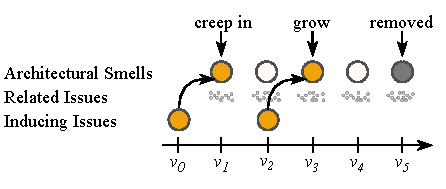
\includegraphics[width=0.8\columnwidth]{picture/lifecycle.pdf}
%    \caption{Lifecycle of architectural smells}
%    \label{fig:v-smell-issue}
%\end{figure}

Understanding \ac{ASI} issues is key to preventing architectural decay at its source.
\autoref{fig:v-smell-issue} illustrates the general life cycle of smells and the distinct temporal opportunities for prevention.
A smell enters the system at $v_1$, expands at $v_3$, and is eventually removed at $v_5$.
Prior research on smell-impacted issues (\tikz[baseline=-0.25em]{
  \node[draw=kit-gray, circle, minimum size=0.75em, inner sep=0, fill=kit-gray50] (c) {};
}) addresses the period from $v_1$ to $v_4$, when smells \textbf{already} exist and affect development work.
In contrast, \ac{ASI} issues (\tikz[baseline=-0.25em]{
  \node[draw=kit-orange, circle, minimum size=0.75em, inner sep=0,
        pattern=north west lines, pattern color=kit-orange] (c) {};
}) occur at $v_0$ and $v_2$, \textbf{before} the smell manifests or expands.
These are the critical intervention points: if developers could be warned of the potential architectural damage an issue might introduce during its planning phase (at $v_0$ or $v_2$), they could make more informed design decisions and potentially avoid introducing or exacerbating smells altogether.
This shift from reactive remediation to proactive prevention represents a fundamental change in how we can manage architectural quality.

To our knowledge, despite their potential value, \acl{ASI}~issues have not been studied in prior work.
This gap motivates our research, which addresses two fundamental questions:
\begin{enumerate}[label=(\roman*)]
    \item \textbf{Identification}: Can we identify which issues in a project's history induced \aclp{AS}?
    \item \textbf{Prediction}: Can we predict whether an issue will induce \aclp{AS} based solely on information available before implementation?
\end{enumerate}





%%%%%%%%%%%%%%%%% Our Approach %%%%%%%%%%%%%%%%%%%%%%
To address the identification challenge, we develop a traceability recovery approach that links \aclp{AS} to their inducing issues.
Our method combines smell evolution analysis with issue-commit links: we track how file-level changes cause smells to evolve across versions, then trace these changes back through the commit history to the issues.
This chain enables us to systematically annotate issues that historically induced \aclp{AS} in a project.

For the prediction challenge, we introduce \textbf{\approach}, a machine learning-based approach that predicts \acl{ASI} issues using only their title and description, information already available at issue creation (\textbf{before code changes}).
\approach leverages \acp{LLM} to extract semantic representations from text, capturing the architectural implications embedded in natural language descriptions.
We explore multiple classifier families to determine which models are most effective at distinguishing \acl{ASI} issues from regular ones.

%%%%%%%%%%%%%%%%% Evaluation %%%%%%%%%%%%%%%%%%%%%%
We evaluate our approach on three open-source projects.
Our identification method successfully traces 60.7\% to 100\% of smells back to smell-inducing issues, demonstrating that architectural decay can be meaningfully related to specific development activities.
For prediction, we compare nine classifiers across three families: traditional machine learning, fine-tuned transformers, and \acp{LLM}, achieving a recall of up to 0.782 with F\textsubscript{1}-scores up to 0.506.
Additionally, we conduct an ablation study to isolate the contributions of different features and to compare semantic representations, demonstrating which signals are most predictive.
For cold-start scenarios, such as a new project with insufficient training data, we conduct a cross-project evaluation to assess our approach's generalizability.  


%%%%%%%%%%%%%%%%%%%% Contributions %%%%%%%%%%%%%%%%%%%%%%%%%
As such, this paper makes the following three contributions:
\begin{enumerate}[leftmargin=*]
    \item An approach to link architectural smells to issues whose implementations have induced those smells.
    \item An issue-based decay prediction approach, \approach.
%    \item An empirical study on the performance of automated classifiers in predicting \acl{ASI} issues.
    \item A replication package containing code, models, datasets, and the dataset construction tool \cite{replication}.
\end{enumerate}
